\documentclass[12pt]{article}
\usepackage{graphicx}
\usepackage{float}
\usepackage{tcolorbox}
\usepackage{amsmath}
\usepackage{amsfonts}
\usepackage{geometry}
\usepackage{fancyhdr}
\usepackage{adjustbox}
\usepackage{imakeidx}
\geometry{a4paper, top=2cm, bottom=2cm, left=1cm, right=1.5cm,  heightrounded, bindingoffset=5mm}
\pagestyle{fancy}
\fancyfoot[RO]{}
\fancyhead[RO]{Calcolo Numerico, Università degli studi di Firenze}
\fancyhead[L]{Alessandro De Cicco, Luca Fumagalli}
\fancyfoot[C]{\thepage}
\graphicspath{ {./immagini/} }
\usepackage{listings}
\usepackage{color} %red, green, blue, yellow, cyan, magenta, black, white
\definecolor{mygreen}{RGB}{28,172,0} % color values Red, Green, Blue
\definecolor{mylilas}{RGB}{170,55,241}

\lstset{
  language=Matlab,
  basicstyle=\ttfamily\footnotesize,
  keywordstyle=\color{blue},
  stringstyle=\color{mylilas},
  commentstyle=\color{mygreen},
  showstringspaces=false,
  numbers=left,
  numberstyle=\tiny,
  numbersep=9pt,
}

\begin{document}

\begin{titlepage}
\centering

\vspace*{20mm}
\textsc{\LARGE Università degli Studi di Firenze}\\[0.5cm]
\textsc{\Large Corso triennale in Informatica}\\[0.5cm]

\vspace{20mm}

\huge Elaborato Calcolo Numerico\\[0.5cm]

\vspace{20mm}
\small Autori

\Large Alessandro De Cicco (matr.7009346) \\ Luca Fumagalli (matr.7004476)\\[0.5cm]

\vspace{10mm}

\large Anno accademico: 2022/2023\\[0.5cm]

\end{titlepage}


\begin{tcolorbox}
\paragraph{Esercizio 1:}
Verificare che:
$$ -\frac{1}{4}f(x-h)-\frac{5}{6}f(x)+\frac{3}{2}f(x+h)-\frac{1}{2}f(x+2h)+\frac{1}{12}f(x+3h)=hf'(x) + O(h^5)$$
\end{tcolorbox}
\paragraph{Soluzione:} 
Innanzitutto per semplificare i calcoli si può raccogliere: 
$$ \frac{1}{12}[-3f(x-h)-10f(x)+18f(x+h)-6f(x+2h)+f(x+3h)]=hf'(x) + O(h^5)$$
Considerando un \(h\) sufficientemente piccolo si può considerare di approssimare la funzione con il polinomio di Taylor
centrato in \(x_0\) con la funzione:
$$ f(x) = \sum_{k=0}^{\infty}{\frac{f^{(k)}(x_0)}{n!}(x-x_0)^k}$$
Basterà approssimare il polinomio al quarto ordine:
$$ f(x) = f(x_0) + f'(x_0)(x-x_0) + \frac{f''(x_0)}{2!}(x-x_0)^2+\frac{f'''(x_0)}{3!}(x-x_0)^3+$$
$$ + \frac{f''''(x_0)}{4!}(x-x_0)^4+O((x-x_0)^5)$$
Da cui si può ricavare:
\begin{equation}
    \begin{aligned}
        & f(x-h) = f(x) - hf'(x) + \frac{h^2}{2}f''(x)- \frac{h^3}{6}f'''(x)+ \frac{h^4}{24}f''''(x_0) + O(h^5)  \\
        & f(x+h) = f(x) + hf'(x) + \frac{h^2}{2}f''(x) + \frac{h^3}{6}f'''(x) + \frac{h^4}{24}f''''(x_0) + O(h^5)  \\
        & f(x+2h) = f(x) + 2hf'(x) + 2h^2f''(x)+ \frac{4}{3}h^3f'''(x)+ \frac{2}{3}h^4f''''(x_0) + O(h^5) \\
        & f(x+3h) = f(x) + 3hf'(x) + \frac{9}{2}h^2f''(x)+ \frac{9}{2}h^3f'''(x)+ \frac{27}{8}h^4f''''(x_0) + O(h^5)  
    \end{aligned}
\end{equation}
Quindi andando a sostituire si ottiene:
\begin{equation}
    \begin{aligned}
        &\frac{-3f(x-h)-10f(x)+18f(x+h)-6f(x+2h)+f(x+3h)}{12}=\\
        &=\frac{(-3-10+18-6+1)f(x) + (3+18-12+3)hf'(x)+(-\frac{3}{2}+9-12+\frac{9}{2})h^2f''(x)}{12}+ \\
        &+ \frac{(\frac{1}{2}+ 3 -8 +\frac{9}{2})h^3f'''(x) + (-\frac{1}{8}+\frac{3}{4} -4 +\frac{27}{8})h^4f''''(x)}{12}=\\
        &=\frac{12hf'(x) + O(h^5)}{12} = hf'(x)+O(h^5)
    \end{aligned}
\end{equation}
\pagebreak

\begin{tcolorbox}
\paragraph{Esercizio 2:}
Matlab utilizza la doppia precisione IEEE. Stabilire, pertanto, il nesso tra la variabile
\textbf{eps} e la precisione di macchina di questa aritmetica.
\end{tcolorbox}
\paragraph{Soluzione:}
Data la funzione \(fl: I \longrightarrow \mathcal{M}\), che associa ad ogni numero reale \(x \in \mathcal{I}\)
, un corrispondente numero di macchina \(fl(x) \in \mathcal{M}\), lo Standard in doppia precisione IEEE prevede la rappresentazione per arrotondamento del numero \(fl(x)\).

Possiamo quindi affermare che se \(x \in \mathcal{I}, x\neq 0\), allora:
$$ fl(x)=x(1+\epsilon_x), \;\;\;\; |\epsilon_x|\leq u$$
In cui:
$$ u = \frac{1}{2}b^{1-m}\;\;\;\; \text{rappresentazione per arrotondamento}$$   
Dove \(b\) è la base, \(m\) è il numero di cifre per la mantissa e \(\epsilon_x\) l'errore relativo di rappresentazione.

Dato che nello standard IEEE in doppia precisione si utilizza la base \(b=2\) e un numero di cifre per la mantissa pari a \(m=53\), avremo che la 
precisione di macchina con rappresentazione per arrotondamento è data da: \(u=2^{-53}\approx 1.1102* 10^{-16}\)

In Matlab, la variabile \textbf{eps} contiene la precisione di macchina in base 10 che coincide con il valore \(u\) nel caso di rappresentazione per troncamento
infatti vale: \(eps=2.2204*10^{-16}\). 

Dato che \textbf{eps} rappresenta quindi, la distanza tra 1 e il successivo numero in virgola mobile, ovvero il valore: \(x=1+u=1+2^{-53}\)
, il quale è rappresentato da \(fl(x)=1\) dato che \(u\leq eps\). 
L'errore relativo commesso su \(x\) perciò è:
$$ |\epsilon_x| =\frac{|fl(x)-x|}{|x|}=\frac{|1-(1+2^{-53})|}{|1+2^{-53}|}=\frac{2^{-53}}{1+2^{-53}} \le 2^{-53}=u \le eps$$
\begin{tcolorbox}
\paragraph{Esercizio 3:} Spiegare il fenomeno della cancellazione numerica. Fare un esempio che la illustri, spiegandone i dettagli.
\end{tcolorbox}
\paragraph{Soluzione:}
La cancellazione numerica si verifica quando si perdono delle cifre significative durante un'operazione di somma algebrica, con addendi quasi opposti.
Questo è dovuto al fatto che la somma è un'operazione malcondizionata ed è possibile studiarlo, verificando il condizionamento di \(y=x_1+x_2,\;\;\; x_1,x_2 \in \mathbb{R} \;\;\;\text{con}\;\; x_1+x_2\neq 0\).

Siano \(\epsilon_1 \;\text{e}\; \epsilon_2\) gli errori relativi sui dati iniziali e considerando che non venga introdotto nessun nuovo errore nel calcolo della somma precedente, si ottiene:
$$ y(1+\epsilon_y)=x_1(1+\epsilon_1)+x_2(1+\epsilon_2)$$
Da cui si può ricavare che:
$$ |\epsilon_y|\leq \frac{|x_1|+|x_2|}{|x_1+x_2|}\epsilon_x\equiv k\epsilon_x \;\;\;\text{con}\;\; \epsilon_x = max\{|\epsilon_1|,|\epsilon_2|\} $$
Il numero \(k\), quindi, indica il numero di condizionamento, che può essere arbitrariamente grande, nel caso di due addendi quasi opposti tra loro. 
Ciò significa che l'operazione di somma tra numeri quasi opposti è malcondizionata.

Per esempio, supponiamo di voler calcolare \(y=0.2345666-0.2345111\equiv 0.0000555\). 
Se utilizziamo una rappresentazione per arrotondamento alla quarta cifra significativa, otteniamo:
$$\tilde{y}=2.346*10^{-1}-2.345*10^{-1} = 1*10^{-4}$$
L'errore relativo che commettiamo su y sarà quindi:
$$|\epsilon_y| = |\frac{5.55*10^{-5}-1*10^{-4}}{5.55*10^{-5}}|\simeq 0.8018$$
Andando quindi a calcolare il numero di condizionamento \(k\), otteniamo:
$$ k=\frac{|x_1|+|x_2|}{|x_1+x_2|}=\frac{|0.2345666|+|-0.2345111|}{|0.2345666-0.2345111|}=8.45*10^3$$
perciò avendo un numero notevolmente alto, la somma precedente è malcondizionata e abbiamo una perdita di cifre significative. 
\begin{tcolorbox}
\paragraph{Esercizio 4:}Scrivere una function Matlab, \texttt{radice(x)} che, avendo in ingresso un numero x non negativo, 
calcoli \(\sqrt[6]{x}\) utilizzando solo operazioni algebriche elementari, con la massima precisione possibile. Confrontare con il risultato fornito da 
\(x^{(1/6)}\) per 20 valori di x, equispaziati logaritmicamente nell’intervallo \([1e-10,1e10]\), tabulando i risultati in modo che si possa verificare che si è ottenuta la massima precisione possibile.
\end{tcolorbox}
\paragraph{Soluzione:}
E' possibile notare che la radice sesta di un numero k sia data dalla soluzione positiva dell'equazione \( x^6 = k \), che può essere riscritta come \( x^6 - n= 0 \).
Ciò equivale a ricercare la radice della funzione nel semiasse positivo delle ascisse della funzione \(f(x)=x^6-k\), è possibile quindi usare il metodo di Newton per trovarla.
Quindi il passo iterativo dell'algoritmo diventa:
$$x_{n+1}=x_n - \frac{f(x_n)}{f'(x_n)} = x_n - \frac{x_n^6 - k}{6x_n^5} = x_n - \frac{1}{6}(x_n - \frac{k}{x_n^5})$$
Da questo risultato si giunge nel formulare il seguente metodo iterativo che converge verso la radice sesta di un numero x:
\begin{enumerate}
    \item Si stima un valore iniziale di partenza \(x_0\)
    \item Dopodiché si pone \(x_{n+1}=x_n + \bigtriangleup x_n\;\; \text{in cui}\;\; \bigtriangleup x_n = (\frac{x}{x^{5}_n}-x_n)\frac{1}{6} \quad \forall n=0,1,2,...\)
    \item Viene reiterato il passo precedente finchè non risulta che la differenza \(|x_{n+1}-x_n|\)  sia minore di una precisione scelta
\end{enumerate}
Traducendo il precedente algoritmo in Matlab, otteniamo il seguente codice:
\begin{lstlisting}[frame=single]
function y = radice(x)
% 
% y = radice(x)
% 
% Calcola la radice sesta di x utilizzando solo operazioni algebriche
% elementari con la massima precisione possibile.
% 
% Input: x, numero di cui calcolare la radice
% Output: y, risultato dell'operazione di radice
%
%

if x<= 0, error("Il radicando non deve essere negativo"); end
x0 = 1;
x1 = x0 + (x/(x0^5)-x0)/6;
err=1;
while err>=eps*(1+abs(x0))
    x0 = x1;
    x1 = x0 + (x/(x0*x0*x0*x0*x0)-x0)/6;
    err=abs(x1-x0);
end
y=x1;
return
end
\end{lstlisting}
Con il seguente codice si vanno a generare 20 valori equispaziati logaritmicamente nell'intervallo \([1e-10,1e10]\) e vengono comparate la rappresentazione esatta della radice con
quella della funzione radice precedente:
\begin{lstlisting}[frame=single]
approssimato = zeros(1,20);
esatto = zeros(1,20);
errore = zeros(1,20);
x = logspace(log10(1e-10),log10(1e10),20);
for i = 1:20
    approssimato(i) = radice(x(i));
    esatto(i) = (x(i))^(1/6);
    errore(i) = abs(approssimato(i)-esatto(i));
end
variabili = {'n', 'approssimato', 'esatto', 'errore'};
table(x',approssimato',esatto', errore','VariableNames',variabili);  
\end{lstlisting}
Si ottengono così i seguenti risultati:
\begin{center}
    \begin{tabular}{||c | c | c | c | c||} 
        \hline
        & n & approssimato & esatto & errore\\
        \hline
        \hline
        1 & 1.0000e-10 & 0.0215 & 0.0215 & 3.4694e-18\\
        \hline
        2 & 1.1288e-09 & 0.0323 & 0.0323 & 6.9389e-18\\
        \hline
        3 & 1.2743e-08 & 0.0483 & 0.0483 & 6.9389e-18\\
        \hline
        4 & 1.4384e-07 & 0.0724 & 0.0724 & 1.3878e-17\\
        \hline
        5 & 1.6238e-06 & 0.1084 & 0.1084 & 2.7756e-17\\
        \hline
        6 & 1.8330e-05 & 0.1624 & 0.1624 & 2.7756e-17\\
        \hline
        7 & 2.0691e-04 & 0.2432 & 0.2432 & 2.7756e-17\\
        \hline
        8 & 0.0023 & 0.3643 & 0.3643 & 0\\
        \hline
        9 & 0.0264 & 0.5456 & 0.5456 & 0\\
        \hline
        10 & 0.2976 & 0.8171 & 0.8171 & 0\\
        \hline
        11 & 3.3598 & 1.2238 & 1.2238 & 0\\
        \hline
        12 & 37.9269 & 1.8330 & 1.8330 & 2.2204e-16\\
        \hline
        13 & 428.1332 & 2.7453 & 2.7453 & 0\\
        \hline
        14 & 4.8329e+03 & 4.1118 & 4.1118 & 8.8818e-16\\
        \hline
        15 & 5.4556e+04 & 6.1585 & 6.1585 & 0\\
        \hline
        16 & 6.1585e+05 & 9.2239 & 9.2239 & 0\\
        \hline
        17 & 6.9519e+06 & 13.8150 & 13.8150 & 0\\
        \hline
        18 & 7.8476e+07 & 20.6914 & 20.6914 & 3.5527e-15\\
        \hline
        19 & 8.8587e+08 & 30.9905 & 30.9905 & 7.1054e-15\\
        \hline
        20 & 1.0000e+10 & 46.4159 & 46.4159 & 7.1054e-15\\
        \hline
    \end{tabular}
\end{center}
E' possibile notare come i valori ottenuti dalla funzione si avvicinino molto ai valori reali, con una tolleranza che è vicina ad \texttt{eps}.
\pagebreak

\begin{tcolorbox}
\paragraph{Esercizio 5:}
Scrivere function Matlab distinte che implementino efficientemente i metodi di Newton e delle secanti per la ricerca degli zeri di una funzione \(f(x)\). 
Per tutti i metodi, utilizzare come criterio di arresto:
$$|x_{n+1} - x_n| \leq tol \cdot (1 + |x_n|)$$
essendo \(tol\) una opportuna tolleranza specificata in ingresso. Curare particolarmente la robustezza del codice.
\end{tcolorbox}
\paragraph{Soluzione:}\mbox{}\\
\texttt{CODICE Matlab per il metodo di Newton}
\begin{lstlisting}[frame=single]
function [x,nit] = newton(f,f1,x0,tolx,maxit)
% Il metodo di Newton serve per determinare una approssimazione della
% radice a partire da un'approssimazione iniziale.
% 
% Input: f = funzione di cui vogliamo trovare la radice
%        f1 = derivata prima della funzione f
%        x0 = approsimazione iniziale della radice
%        tolx = tolleranza fissata
%        maxit = massimo numero di iterazioni fissato
%
% Output: x = radice della funzione f
%         nit = numero di iterazioni svolte, vale -1 se la tolleranza non 
%         e' soddisfatta entro maxit o la derivata si annulla
%
if nargin<4, error('Argomenti in input non sufficienti')
elseif nargin==4, maxit=100;end
if tolx<eps, error('Tolleranza non valida');end

x=x0;
nit=-1;
for i=1:maxit
    fx = feval(f,x);
    f1x = feval(f1,x);
    if f1x == 0, error('Derivata prima uguale a 0'); end
    x = x - fx/f1x;
    if abs(x-x0)<=tolx * (1+abs(x0))
        nit=i;
        break;
    else
        x0 = x;
    end
end

if nit == -1, disp('Tolleranza desiderata non raggiunta');end
return
end 
\end{lstlisting}
\texttt{CODICE Matlab per il metodo delle secanti}
\begin{lstlisting}[frame=single]
function [x,nit] = secanti(f,x0,x1,tolx,maxit)
% 
% Il metodo delle secanti serve per determinare una approssimazione della
% radice di f(x)=0 a partire da due valori iniziali x0 e x1.
% 
% Input: f = funzione di cui vogliamo trovare la radice
%        x0 = approsimazione iniziale della radice
%        x1 = approsimazione iniziale della radice
%        tolx = tolleranza fissata
%        maxit = massimo numero di iterazioni fissato
%
% Output: x = radice della funzione f
%         nit = numero di iterazioni svolte, vale -1 se la tolleranza non
%         e' soddisfatta entro maxit o la derivata si annulla
%
if nargin<4, error('Argomenti in input non sufficienti')
elseif nargin==4, maxit=100;end
if tolx<eps, error('Tolleranza non valida');end
nit=-1;
for i=1:maxit
    fx0 = feval(f,x0);
    fx1 = feval(f,x1);
    if fx1-fx0 == 0, error('Il denominatore e'' uguale a 0');end
    x = (fx1*x0-fx0*x1)/(fx1-fx0);
    x0 = x1;
    x1 = x;
    if abs(x-x0)<=tolx * (1+abs(x0))
        nit=i;
        break;
    end
end

if nit == -1, disp('Tolleranza desiderata non raggiunta');end
return
end
\end{lstlisting}
\begin{tcolorbox}
\paragraph{Esercizio 6:}Utilizzare le \(function\) del precedente esercizio per determinare una approssimazione della radice della funzione:
$$f(x)=x-cos(x)$$
per \(tol = 10^{-3}, 10^{-6}, 10^{-9}, 10^{-12}\), partendo da \(x_0 = 0\) (e \(x_1 = 0.1\) per il metodo delle secanti). 
Tabulare i risultati, in modo da confrontare il costo computazionale di ciascun metodo.
\end{tcolorbox}
\paragraph{Soluzione:}

\begin{center}
    \begin{tabular}{|| c || c | c || c | c||} 
        \hline
        tol & Radici Newton & iterazioni & Radici secanti & iterazioni\\
        \hline
        \(10^{-3}\) & 7.390851333852840e-01 & 4 & 7.390985629062998e-01 & 4\\
        \hline
        \(10^{-6}\) & 7.390851332151607e-01 & 5 & 7.390851332151466e-01 & 6\\
        \hline
        \(10^{-9}\) & 7.390851332151607e-01 & 5 & 7.390851332151607e-01 & 7\\
        \hline
        \(10^{-12}\) & 7.390851332151607e-01 & 6 & 7.390851332151607e-01 & 7\\
        \hline
    \end{tabular}
\end{center}
Considerando che per ciascuna iterazione del metodo di Newton si eseguono 2 valutazioni funzionali mentre per il metodo delle secanti ne viene fatta solo una,
si ottiene che Newton utilizza un costo computazionale maggiore rispetto al metodo delle secanti in questo caso.
\newpage
\begin{tcolorbox}
\paragraph{Esercizio 7:}Utilizzare le \(function\) dell'Esercizio 5 per determinare una approssimazione della radice della funzione:
$$f(x)=[x-cos(x)^5]$$
per \(tol = 10^{-3}, 10^{-6}, 10^{-9}, 10^{-12}\), partendo da \(x_0 = 0\) (e \(x_1 = 0.1\) per il metodo delle secanti). 
Tabulare i risultati, in modo da confrontare il costo computazionale e l’accuratezza di ciascun metodo. Commentare i risultati ottenuti.\pagebreak
\end{tcolorbox}
\paragraph{Soluzione:}
\begin{center}
    \begin{tabular}{|| c || c | c || c | c||} 
        \hline
        tol & Radici Newton & iterazioni & Radici secanti & iterazioni\\
        \hline
        \(10^{-3}\) & 0.732640697751109 & 20 & 0.730145017727562 & 26\\
        \hline
        \(10^{-6}\) & 0.739078762321033 & 51 & 0.739075266476228 & 70\\
        \hline
        \(10^{-9}\) & 0.739085126905744 & 82 & 0.739085038011533 & -1\\
        \hline
        \(10^{-12}\) & 0.7390851331015 & -1 & 0.739085038011533 & -1\\
        \hline
    \end{tabular}
\end{center}
Com'è possibile notare dai precedenti risultati, in entrambi i metodi, essendo la funzione una radice multipla, si eseguono molte più iterazioni rispetto alla funzione 
dell'Esercizio 6, in alcuni casi neanche convergono.
In particolare risulta che il metodo di Newton non converga su tolleranza pari a \texttt{1e-12} mentre il metodo delle secanti non converga nel caso la tolleranza sia pari a:
\texttt{1e-9, 1e-12}.

In conclusione, in caso di radici multiple, non porta alcun vantaggio utilizzare metodi diversi da quello di Newton, anzi avremo un aumento considerevole nel numero di iterazioni.
\begin{tcolorbox}
\paragraph{Esercizio 8:}Scrivere una function Matlab,\\
\texttt{function x = mialu(A,b)}\\
che, data in ingresso una matrice \(A\) ed un vettore \(b\), calcoli la soluzione del sistema lineare \(Ax = b\) con il metodo di fattorizzazione \(LU\) 
con \textit{pivoting parziale}. Curare particolarmente la scrittura e l’efficienza della function, e validarla su due esempi non banali, generati casualmente, 
di cui sia nota la soluzione.
\end{tcolorbox}
\paragraph{Soluzione:}
\texttt{CODICE Matlab per funzione mialu}
\begin{lstlisting}[frame=single]
function x = mialu(A,b)
% x = mialu(A,b)
% data in ingresso una matrice A ed un vettore b, calcoli la soluzione del 
% sistema lineare Ax = b con il metodo di fattorizzazione LU con pivoting 
% parziale. 
% Input: A = matrice in ingresso che va fattorizzata LU con il metodo di 
%            pivoting parziale
%        b = vettore dei termini noti
% Output: x = vettore soluzione di Ax=b
%

[m,n] = size(A);
dimb = length(b);
if m ~= n 
    error("La matrice dei coefficenti A deve essere quadrata")
end
if m ~= dimb
    error("La matrice A ed il vettore b hanno dimensioni discordanti")
end
p = [1:n];
for i =1:n-1
    [mi,ki] = max(abs(A(i:n,i)));
    if mi == 0
        error('La matrice non puo'' essere singolare');
    end
    ki = ki + i - 1;
    if ki > i 
        % inverto la riga i-esima e ki-esima
        A([i,ki],:) = A([ki,i],:);
        % stessa cosa nel vettore delle permutazioni
        p([i,ki]) = p([ki,i]);
    end
    A(i+1:n,i) = A(i+1:n,i)/A(i,i);
    A(i+1:n,i+1:n) = A(i+1:n,i+1:n) - A(i+1:n,i)*A(i,i+1:n);
end
x = b(p);
for i = 1:n
    x(i+1:n) = x(i+1:n)-A(i+1:n,i)*x(i);
end
x(n) = x(n)/A(n,n);
for i = n-1:-1:1
    x(1:i) = x(1:i) - A(1:i,i+1)*x(i+1);
    x(i) = x(i)/A(i,i);
end
return
end
\end{lstlisting}
\textbf{Esempi:}
\begin{equation}A=
    \begin{pmatrix}
        -3 & 5 & -4 \\
        3 & -3 & -4 \\
        -1 & -3 & 4 
    \end{pmatrix}\;\;\;\;\;x=
    \begin{pmatrix}
        1 \\
        1 \\
        -4  
    \end{pmatrix}\;\;\;\;\;b=
    \begin{pmatrix}
        18 \\
        16\\
        -20  
    \end{pmatrix}
\end{equation}
\begin{equation}
    A=
    \begin{pmatrix}
        3 & -1 & 1 & 1 \\
        0 & 3 & -3 & 2 \\
        2 & 2 & 2 & 2 \\
        -3 & 3 & 3 & -1 \\
    \end{pmatrix}\;\;\;\;\;x=
    \begin{pmatrix}
        1 \\
        -2 \\
        1 \\
        -3 
    \end{pmatrix}\;\;\;\;\;b=
    \begin{pmatrix}
        3 \\
        -15 \\
        -6 \\
        -3 
    \end{pmatrix}
\end{equation}
In entrambi i casi sono stati creati i valori della matrice \(A\) e del vettore \(x\) in modo casuale, mentre il vettore dei termini noti \texttt{b}, è stato calcolato tramite il prodotto
\texttt{A*x}. Una volta inseriti i valori di \texttt{A} e \texttt{b} nella funzione \texttt{mialu(A,b)}, questa ha restituito il vettore x correttamente.
\newpage
\begin{tcolorbox}
\paragraph{Esercizio 9:}Scrivere una function Matlab,\\
\texttt{function x = mialdl(A,b)}\\
che, data in ingresso una matrice \(A\) ed un vettore \(b\), calcoli la soluzione del corrispondente sistema lineare utilizzando la fattorizzazione \(LDL^{T}\). Curare particolarmente la scrittura e l’efficienza della function, e validarla su due esempi non banali, generati casualmente, 
di cui sia nota la soluzione.
\end{tcolorbox}
\paragraph{Soluzione:}

\texttt{CODICE Matlab per funzione mialdl}
\begin{lstlisting}[frame=single]
function x = mialdl(A,b)
% x = mialdl(A,b)
% data in ingresso una matrice A ed un vettore b, calcoli la soluzione del 
% sistema lineare Ax = b con il metodo di fattorizzazione LDL^T.

% Input: A = matrice in ingresso che va fattorizzata LDL^T
%        b = vettore dei termini noti
% Output: x = vettore soluzione di Ax=b
%
[m,n] = size(A);
dimb = length(b);
if m ~= n 
    error("La matrice dei coefficenti A deve essere quadrata")
end
if m ~= dimb
    error("La matrice A ed il vettore b hanno dimensioni discordanti")
end
if A(1,1) <= 0, error('la matrice non e'' sdp'); end
A(2:n,1) = A(2:n,1)/A(1,1);
for j = 2:n
    v = (A(j,1:j-1).') .* diag(A(1:j-1,1:j-1));
    A(j,j) = A(j,j) - A(j,1:j-1)*v;
    if A(j,j) <= 0, error('la matrice non e'' sdp'); end
    A(j+1:n,j) = (A(j+1:n,j) - A(j+1:n,1:j-1) * v)/A(j,j);
end
x = b;
for i=1:n
    x(i+1:n) = x(i+1:n)-(A(i+1:n,i)*x(i));
end
x = x./diag(A);
for i=n:-1:2
    x(1:i-1) = x(1:i-1)-A(i,1:i-1).'*x(i);
end 
end
\end{lstlisting}
\textbf{Esempi:}
\begin{equation}A=
    \begin{pmatrix}
        5 & 3 & -1 \\
        3 & 6 & -1 \\
        -1 & -1 & 6 
    \end{pmatrix}\;\;\;\;\;x=
    \begin{pmatrix}
        -3 \\
        0\\
        0  
    \end{pmatrix}\;\;\;\;\;b=
    \begin{pmatrix}
        -15 \\
        -9 \\
        3  
    \end{pmatrix}
\end{equation}
\begin{equation}
    A=
    \begin{pmatrix}
        3 & -2 & 1 & 0 \\
        -2 & 4 & 2 & 0 \\
        1 & 2 & 5 & -3 \\
        0 & 0 & -3 & 5 \\
    \end{pmatrix}\;\;\;\;\;x=
    \begin{pmatrix}
        1 \\
        1 \\
        -2 \\
        1 
    \end{pmatrix}\;\;\;\;\;b=
    \begin{pmatrix}
        -1 \\
        -2 \\
        -4 \\
        1 
    \end{pmatrix}
\end{equation}
In entrambi i casi sono stati creati i valori della matrice \(A\) e del vettore \(x\) in modo casuale, mentre il vettore dei termini noti \texttt{b}, è stato calcolato tramite il prodotto
\texttt{A*x}. Una volta inseriti i valori di \texttt{A} e \texttt{b} nella funzione \texttt{mialdl(A,b)}, questa ha restituito il vettore x correttamente.
\begin{tcolorbox}
\paragraph{Esercizio 10:}Scrivere una function Matlab,\\
\texttt{function [x,nr] = miaqr(A,b)}\\
che, data in ingresso la matrice \(A\;m \times  n\), con \(m \geq n = rank(A)\), ed un vettore \(b\) di lunghezza  \(m\), calcoli la soluzione del sistema lineare \(Ax = b\) nel senso dei minimi quadrati e, inoltre, 
la norma, \(nr\), del corrispondente vettore residuo. Curare particolarmente la scrittura e l’efficienza della function. Validare la function miaqr su due esempi non banali, generati casualmente, 
confrontando la soluzione ottenuta con quella calcolata con l’operatore Matlab \(\setminus\) 
\end{tcolorbox}
\paragraph{Soluzione:}

\texttt{CODICE Matlab per funzione mialdl}
\begin{lstlisting}[frame=single]
function [x,nr] = miaqr(A,b)
%
% [x,nr] = miaqr(A,b)
%
% La funzione miaqr fattorizza QR la matrice in ingresso A, dopodiche'  
% restituisce la soluzione x del sistema Ax=b insieme alla norma del
% vettore residuo
% 
% Input: A = matrice in ingresso
%        b = vettore dei termini noti
% Output: x = soluzione del sistema
%         nr = norma del vettore residuo
%

[m,n] = size(A);
dimb = length(b);
if n > m, error('Dimensioni matrice A errate'); end
if dimb ~= m, error('Dimensione vettore dei termini noti sbagliata'); end
for i=1:n
    alfa = norm(A(i:m,i));
    if alfa == 0, error('La matrice non ha rango massimo'), end
    if A(i,i) >= 0, alfa = -alfa; end
    v1 = A(i,i) - alfa;
    A(i,i) = alfa;
    A(i+1:m,i) = A(i+1:m,i)/v1;
    beta = -v1/alfa;
    A(i:m,i+1:n) = A(i:m,i+1:n) - (beta*[1; A(i+1:m,i)])*...
        ([1; A(i+1:m,i)]' * A(i:m,i+1:n));
end
for i=1:n
    v = [1; A(i+1:m,i)];
    beta = 2/(v'*v);
    b(i:dimb) = b(i:dimb) - (beta*(v'*b(i:dimb)))*v;
end
for i=n:-1:1
    b(i) = b(i)/A(i,i);
    b(1:i-1) = b(1:i-1) - A(1:i-1,i)*b(i);
end
x = b(1:n);
nr = norm(b(n+1:m));
end
\end{lstlisting}
\textbf{Esempio 1:}
Data la matrice A di dimensioni \(4 \times 3\) e il vettore b (entrambi generati casulmente):
\begin{equation}A=
    \begin{pmatrix}
        4 &	-5 & 2 \\
        3 & -5 & -4 \\
        3 & 3 & 2 \\
        -5 & 5 &-4
    \end{pmatrix}\;\;\;\;\;
    b=
    \begin{pmatrix}
        -8\\
        3\\
        -4\\
        3 
    \end{pmatrix}
\end{equation}
La soluzione generata dalla \texttt{function miaqr} è:
\begin{equation*}xMiaqr=
    \begin{pmatrix}
        -5.4619e-01\\
        -4.1315e-02\\
        -9.0373e-01
    \end{pmatrix}\text{, con norma }\;\; nr = 5.3356e-00
\end{equation*}
Mentre la soluzione generata da \(x=A\setminus b\) è:
\begin{equation*} x=
    \begin{pmatrix}
        -5.4619e-01\\
        -4.1315e-02\\
        -9.0373e-01
    \end{pmatrix}
\end{equation*}
\textbf{Esempio 2:}
Data la matrice A di dimensioni \(5 \times 4\) e il vettore b (entrambi generati casulmente):
\begin{equation}A=
    \begin{pmatrix}
        3 & 2 & -2 & -4 \\
        -3 & 0 & -3 & -4 \\
        -1 & -4 & 0 & 3 \\
        1 & 3 & -4 & -2 \\
        -3 & -4 & -1 & 1 
    \end{pmatrix}\;\;\;\;\;
    b=
    \begin{pmatrix}
        10\\
        -1\\
        4\\
        5 \\
        -1
    \end{pmatrix}
\end{equation}
La soluzione generata dalla \texttt{function miaqr} è:
\begin{equation*}xMiaqr=
    \begin{pmatrix}
        2.8454e+00\\
        -1.8283e+00\\
        -1.7138e+00\\
        -4.5249e-01
    \end{pmatrix}\text{, con norma }\;\; nr = 1.4966e+00
\end{equation*}
Mentre la soluzione generata da \(x=A\setminus b\) è:
\begin{equation*} x=
    \begin{pmatrix}
        2.8454e+00\\
        -1.8283e+00\\
        -1.7138e+00\\
        -4.5249e-01
    \end{pmatrix}
\end{equation*}
\begin{tcolorbox}
\paragraph{Esercizio 11:}Data la function Matlab \\
\begin{lstlisting}[frame=single]
function [A1,A2,b1,b2] = linsis(n,simme)
%
%
rng(0);
[q1,r1] = qr(rand(n));
if nargin==2
    q2 = q1'; 
else
    [q2,r1] = qr(rand(n));
end
A1 = q1*diag([1 2/n:1/n:1])*q2;
A2 = q1*diag([1e-10 2/n:1/n:1])*q2;
b1 = sum(A1,2);
b2 = sum(A2,2);
return
\end{lstlisting}
che crea sistemi lineari casuali di dimensione n con soluzione nota,
$$A_1x = b_1,\;\;\; A_2x = b_2, \;\;\;x = (1,...,1)^T \in \mathbb{R}^n,$$
risolvere, utilizzando la \textit{function} \texttt{mialu}, i sistemi lineari generati da \texttt{[A1,A2,b1,b2]=linsis(5)}. 
Commentare l’accuratezza dei risultati ottenuti, dandone spiegazione esaustiva.
\end{tcolorbox}
\paragraph{Soluzione:}
Innanzitutto bisogna notare che eseguendo la function \texttt{linsis(5)}, che ha in input un solo argomento, andiamo a creare matrici non simmetriche. 
Perciò utilizzando i risultati come input della \textit{function} \texttt{mialu}, otteniamo i seguenti risultati:
\begin{enumerate}
    \item Nel primo caso, ovvero calcolando \texttt{x1 = mialu(A1,b1)}, il vettore risultante è: 
    \begin{equation*} x_1=
        \begin{pmatrix}
            9.999999999999999e-01\\
            9.999999999999998e-01\\
            9.999999999999998e-01\\
            1\\
            9.999999999999998e-01
        \end{pmatrix}
    \end{equation*}
    Il risultato è pressoché identico al risultato atteso. D'altra parte il numero di condizionamento \(K\) della matrice A1, dato dalla funzione \texttt{cond(A1)}
    è pari a \(K = 2.5000e+00\). Ciò significa che il problema è quindi ben condizionato, essendo \(K\) piccolo.
    \item Nel secondo caso invece, ovvero calcolando \texttt{x2 = mialu(A2,b2)}, il vettore risultante è:
    \begin{equation*} x_2=
        \begin{pmatrix}
            9.999996476574766e-01\\
            1.000000446226050e+00\\
            1.000000098875194e+00\\
            1.000000207059384e+00\\
            1.000000011600807e+00
        \end{pmatrix}
    \end{equation*}
    Il cui numero di condizionamento della matrice A2, dato dalla funzione \texttt{cond(A2)} è pari a \(K = 9.999995892902628e+09\). Dato che il numero ottenuto è molto 
    grande, significa che il problema risulta mal condizionato. \\
    Questo è dovuto all'operazione con cui otteniamo la matrice A2, in particolare all'operazione: \texttt{ diag ([1e-10 2/n:1/n:1])}, in cui il primo elemento della matrice 
    diagonale è molto vicino allo zero:
    \begin{equation*} D=
        \begin{pmatrix}
            1e-10 & 0 & 0 & 0 & 0 \\
            0 & 0.4 & 0 & 0 & 0 \\
            0 & 0 & 0.6 & 0 & 0 \\
            0 & 0 & 0 & 0.8 & 0 \\
            0 & 0 & 0 & 0 & 1
        \end{pmatrix}\;\;\;\;\;
    \end{equation*}
    Infatti, ricordando la costruzione della matrice A2 mediante \(A=Q_1 * D * Q_2\), 
    per calcolare la matrice inversa basterà ricordare che \(Q_1\) e \(Q_2\) sono matrici ortogonali, ottendendo:
    \(A^{-1}=Q_2^{-1} * D^{-1} * Q_1^{-1} = Q_2^{T} * D^{-1} * Q_1^{T}\).\\
    Inoltre si può notare che la matrice inversa di una matrice diagonale è una matrice diagonale dove gli elementi diagonali sono il reciproco rispetto alla matrice di partenza:
    \begin{equation*} D^{-1}=
        \begin{pmatrix}
            1e10 & 0 & 0 & 0 & 0 \\
            0 & 2.5 & 0 & 0 & 0 \\
            0 & 0 & 1.667 & 0 & 0 \\
            0 & 0 & 0 & 1.25 & 0 \\
            0 & 0 & 0 & 0 & 1
        \end{pmatrix}\;\;\;\;\;
    \end{equation*}
    Calcolando quindi la matrice inversa con la formula sopra illustrata si ottiene che 
    moltiplicando \(Q_{1}^{T}\) per \(D\) si realizza una matrice dove la prima colonna avrà elementi nell'ordine di \(1e9\), 
    tale matrice moltiplicata per \(Q_2^{T}\) infine produce una matrice dove tutti gli elementi 
    raggiungono valori molto elevati, come si può notare dalla norma della matrice inversa:
    \begin{equation*}
    \Arrowvert A1 \Arrowvert_{2}=1 \qquad
    \Arrowvert A2 \Arrowvert_{2}=1 \qquad
    \Arrowvert A1^{-1} \Arrowvert_{2}=2.5 \qquad
    \Arrowvert A2^{-1} \Arrowvert_{2}=1.0000e+10
    \end{equation*}
    Da questi risultati si evince quindi che la costruzione di A2 risulta peggiore rispetto a quella di A1 visto che risulta più sensibile ad errori.
\end{enumerate}
\begin{tcolorbox}
\paragraph{Esercizio 12:} Risolvere, utilizzando la \textit{function} \texttt{mialdlt}, i sistemi lineari generati da\\ \texttt{[A1,A2,b1,b2]=linsis(5,1)}. 
Commentare l’accuratezza dei risultati ottenuti, dandone spiegazione esaustiva.   
\end{tcolorbox}
\paragraph{Soluzione:}
Similmente al caso precedente usando la \textit{function} \texttt{mialdlt}, otteniamo i seguenti risultati:
\begin{enumerate}
    \item Nel primo caso, ovvero calcolando \texttt{x1 = mialdlt(A1,b1)}, il vettore risultante è: 
    \begin{equation*} x_1=
        \begin{pmatrix}
            1\\
            9.999999999999994e-01\\
            9.999999999999999e-01\\
            1.000000000000000e+00\\
            1.000000000000000e+00
        \end{pmatrix}
    \end{equation*}
    Il risultato è pressoché identico al risultato atteso. D'altra parte il numero di condizionamento \(K\) della matrice A1, dato dalla funzione \texttt{cond(A1)}
    è pari a \(K = 2.5000e+00\), quindi il problema è  ben condizionato.
    \item Nel secondo caso invece, ovvero calcolando \texttt{x2 = mialdlt(A2,b2)}, il vettore risultante è:
    \begin{equation*} x_2=
        \begin{pmatrix}
            1.000000052293492e+00\\
            1.000000058138759e+00\\
            1.000000008150719e+00\\
            1.000000058625536e+00\\
            1.000000040588329e+00
        \end{pmatrix}
    \end{equation*}
    Il cui numero di condizionamento della matrice A2, dato dalla funzione \texttt{cond(A2)} è pari a \(K = 9.999995645805687e+09\). Dato che il numero ottenuto è molto 
    grande significa che il problema è mal condizionato. \\
    Tuttavia a differenza del caso precedente vengono costruite matrici simmetriche definite positive infatti:
    \begin{itemize}
        \item costruendo la matrice con \(Q_1 * D * Q_1^{T}\) si ha che la transposta è data data da: \((Q_1 * D * Q_1^{T})^{T}=Q_1*D^{T}*Q_1^{T}=Q_1 * D * Q_1^{T}\). 
        \item \(\forall x \in R^{n}, xQ_1 * D * Q_1^{T}x^{T} = (xQ_1) * D * (xQ_1)^{T}\), sostituendo \(xQ_1=y \in R^{n}\) con \(y \ne 0\) 
        (perché la matrice \(Q_1\) è non singolare ), avremo che \(y*D*y^{T}>0\) perchè gli elementi della matrice diagonale sono tutti positivi, e quindi la matrice è definita positiva
    \end{itemize}
    Questa costruzione ha anche un'altra particolarità, ovvero le matrici A1 e A2 sono simili alla matrice D. Infatti per definizione,
    la matrice A e B sono simili se esiste una matrice P invertibile tale che: \(A=P^{-1}*B*P\). Considerando \(P=Q_1^{T}\) e \(B=D\) 
    allora si ha che: \(A=(Q_1^{T})^{-1}*D*Q_1^{T} = (Q_1^{-1})^{T}*D*Q_1^{T} = (Q_1^{T})^{T}*D*Q_1^{T} = Q_1*D*Q_1^{T}\). 
    Quindi ciò comporta che le matrici A1 e A2 hanno gli stessi autovalori, e quindi lo stesso raggio spettrale della matrice diagonale.
    Anche la matrice inversa di A1 e A2 risulta essere simile, come si può notare anche da \(A^{-1}=(Q_1^{T})*D^{-1}*Q_1\).
    Quindi in generale avremo che: 
    \begin{equation*}
        \begin{aligned}
            & \Arrowvert A_1 \Arrowvert \ge \rho(D_1) = 1  \\
            & \Arrowvert A_1^{-1} \Arrowvert \ge \rho(D_1^{-1}) = 2.5 \\
            & \Arrowvert A_2 \Arrowvert \ge \rho(D_2) = 1  \\
            & \Arrowvert A_2^{-1} \Arrowvert \ge \rho(D_2^{-1}) = 1e10  \\
        \end{aligned}
    \end{equation*}
    Per cui data una norma qualsiasi, abbiamo che il numero di condizionamento della prima matrice sarà 
    \(\Arrowvert A_1 \Arrowvert * \Arrowvert A_1^{-1} \Arrowvert \ge 2.5\), mentre per la seconda 
    \(\Arrowvert A_2 \Arrowvert * \Arrowvert A_2^{-1} \Arrowvert \ge 1e10\). 
    Ciò tuttavia è vero solo in condizioni ottimali, infatti entrambe le matrici 
    sono soggette ad errori di round-off dovuti alla loro costruzione.
    Ciò si può notare anche solo usando il comando \texttt{isSymmetric()}
    che per entrambe le matrici risulta essere falso, si può anche notare come il 
    numero di condizionamento della seconda matrice calcolato 
    tramite Matlab va in contraddizione con quanto stabilito.
    Quindi il mal condizionamento del secondo sistema rispetto al primo, causa errori di imprecisione maggiori.

\end{enumerate}

\begin{tcolorbox}
\paragraph{Esercizio 13:}Utilizzare la \textit{function} \texttt{miaqr} per risolvere, nel senso dei minimi quadrati, i sistemi lineari sovradeterminati\\
\texttt{Ax = b, \;\;\;\;\;\;(D*A)x = (D*b),\;\;\;\;\;\; (D1*A)x = (D1*b),}\\
definiti dai seguenti dati:\\\\
\texttt{
A = [ 1 3 2; 3 5 4; 5 7 6; 3 6 4; 1 4 2 ]; \\
b=[15 28 41 33 22]';\\
D = diag(1:5);\\
D1 = diag(pi*[1 1 1 1 1]).}\\\\
Calcolare le corrispondenti soluzioni e residui, e commentare i risultati ottenuti.
\end{tcolorbox}
\paragraph{Soluzione:}
Ricordando che risolvere il sistema nel senso dei minimi quadrati consiste in un problema di ottimizzazione nella forma:
$$\min_{x \in \mathbb{R}^n}\Arrowvert Ax-b \Arrowvert_{2}^2$$
dove per residuo si intente un vettore  \(r=Ax-b\), si nota che la norma euclidea al quadrato dei residui non è altro che il valore all'ottimo. 
Applicando quindi la \textit{function} \texttt{miaqr} ai vari sistemi, si ottengono quindi le seguenti soluzioni, residui e norme euclidee al quadrato:
\begin{equation*} x_1=
    \begin{pmatrix}
        3.000000000000008e+00\\
        5.800000000000001e+00\\
        -2.500000000000008e+00
    \end{pmatrix}
    ;  r_1=
    \begin{pmatrix}
        0.399999999999993\\
        -3.5527136788005e-15\\
        -0.399999999999999\\
        0.799999999999997\\
        -0.800000000000004
    \end{pmatrix}
    ;  \Arrowvert r_1 \Arrowvert_{2}^2 = 1.6
\end{equation*}
\begin{equation*} x_2=
    \begin{pmatrix}
        -6.025699862322442e-01\\
        4.701698026617703e+00\\
        1.758375401560388e+00
    \end{pmatrix}
    ;  r_2=
    \begin{pmatrix}
        2.01927489674164\\
        1.46856356126666\\
        -1.65213400642492\\
        1.74391922900415\\
        -1.3951353832033
    \end{pmatrix}
    ;  \Arrowvert r_2 \Arrowvert_{2}^2 = 13.9513538320331 
\end{equation*}
\begin{equation*} x_3=
    \begin{pmatrix}
        3.00000000000001\\
        5.80000000000001\\
        -2.50000000000003
    \end{pmatrix}
    ;  r_3=
    \begin{pmatrix}
        1.25663706143589\\
        -5.6843418860808e-14\\
        -1.25663706143598\\
        2.51327412287179\\
        -2.51327412287183
    \end{pmatrix}
    ;  \Arrowvert r_3 \Arrowvert_{2}^2 = 15.7913670417428
\end{equation*}

 Dai risultati ottenuti è possibile notare una grande discrepanza tra quelli ottenuti con il primo e il secondo sistema, nonostante che risolvere il sistema lineare \texttt{Ax=b}
 sia equivalente a risolvere il sistema lineare \texttt{(D*A)x = (D*b)}. Tuttavia possiamo notare che nel caso dei minimi quadrati ciò non è sempre vero. Infatti il problema di minimo nel secondo caso risulta essere:
 $$\min_{x \in \mathbb{R}^n}\Arrowvert (D*A)x-(D*b) \Arrowvert_{2}^2 = \min_{x \in \mathbb{R}^n} \Arrowvert D*(Ax-b) \Arrowvert_{2}^2$$
 Non è detto infatti che la soluzione \(x_1\) risolva questo nuovo problema, anzi, provando a sostituire \(x_1\) nel secondo sistema si ottiene come risultato
 che la funzione obiettivo ha come valore \(27.8400000000001\) che risulta essere una soluzione ben peggiore rispetto a quella data da \(x_2\). \\
 Nel caso invece del terzo sistema, possiamo notare che la matrice altro non è che il risultato del prodotto \(\pi*I\).
Il problema in questo caso risulterà essere:
$$\min_{x \in \mathbb{R}^n}\Arrowvert (\pi*A)x-(\pi*b) \Arrowvert_{2}^2 = \min_{x \in \mathbb{R}^n} \Arrowvert \pi*(Ax-b) \Arrowvert_{2}^2 =\pi^2 * \min_{x \in \mathbb{R}^n} \Arrowvert Ax-b \Arrowvert_{2}^2 $$
E' possibile notare che tale problema equivale a quello del primo sistema moltiplicato per uno scalare, per cui la soluzione di questo problema di minimo coincide con la soluzione di quella del primo sistema. Infatti le due soluzioni ad eccezzione di qualche decimale coincidono, come si può inoltre notare dalla norma residua calcolata
ponendo \(x = x_1\) che risulta essere: \(15.7913670417428\), le cifre inesatte sono dovute da piccole imprecisioni delle operazioni in artimetica finita, specialmente considerando l'approssimazione necessaria di \(\pi\), non essendo possible rappresentare il numero interamente in codice macchina.



\newpage
\begin{tcolorbox}
\paragraph{Esercizio 14:}Scrivere una function Matlab,\\
\texttt{[x,nit] = newton(fun,jacobian,x0,tol,maxit)}\\
che implementi efficientemente il metodo di Newton per risolvere sistemi di equazioni nonlineari. 
Curare particolarmente il criterio di arresto, che deve essere analogo a quello usato nel caso scalare. 
La seconda variabile, se specificata, ritorna il numero di iterazioni eseguite. Prevedere opportuni valori 
di \textit{default} per gli ultimi due parametri di ingresso.
\end{tcolorbox}
\paragraph{Soluzione:} Funzione che calcola  il metodo di Newton per risolvere sistemi di equazioni nonlineari
\begin{lstlisting}[frame=single]
function [x,nit] = newton(fun,jacobian,x0,tol,maxit)
%   [x,nit] = newton(fun,jacobian,x0,tol,maxit)
%   Funzione che implementa il metodo di Newton per sistemi 
%   di equazioni nonlineari
%   
%   Input:
%   fun: function funzione di un sistema nonlineare
%   jacobian: matrice jacobiana di fun
%   x0: approssimazione iniziale
%   tol: tolleranza richiesta
%   maxit: massimo numero di iterazioni richiesto
%   Output:
%   x: risultato del metodo di Newton
%   nit: numero di iterazioni effettuate
%
if nargin < 3
    error('numero argomenti insufficienti');
elseif nargin==3
    tol=1e-13;
    maxit=10e3;
elseif nargin==4
    maxit=10e3;
end
x=x0;
nit=-1;
if tol<0
    error('la tolleranza non puo essere negativa');
end
if maxit<=0
    error('maxit deve essere maggiore di 0');
end
[n,m] = size(jacobian);
nf = size(fun);
if (n~=m)
    error('La matrice Jacobiana deve essere quadrata');
end
if n~=nf
    error('Il numero di righe del vettore fun e della Jacobiana sono diversi');
end
for i=1:maxit
    fx = feval(fun,x);
    f1x = feval(jacobian,x);
    dx=-f1x\(fx);
    x = x + dx;
    if norm(dx./(1+abs(x)),Inf)<=tol
        nit=i;
        break;
    end
end

if nit == -1, disp('Il metodo di Newton per il sistema lineare non converge');end
return
end  
\end{lstlisting}



\newpage
\begin{tcolorbox}
\paragraph{Esercizio 15:} Usare la function del precedente esercizio per risolvere, a partire dal vettore iniziale nullo, 
il sistema nonlineare derivante dalla determinazione del punto stazionario della funzione:  
\begin{equation*} 
    f(\boldsymbol{x})=\frac{1}{2}\boldsymbol{x}^TQ\boldsymbol{x}-\boldsymbol{e}^T\left[ \sin(\frac{\pi}{2}\boldsymbol{x})+\boldsymbol{x}\right],\;\;\;\;\;\;
    \boldsymbol{e}=\frac{1}{100}
    \begin{pmatrix}
        1\\
        2\\
        \vdots \\
        100
    \end{pmatrix}
    \in \mathbb{R}^{100},
\end{equation*}
\begin{equation*}
    Q=
    \begin{pmatrix}
        2 & 1 &  & \\
        1 & \ddots &\ddots& \\
        &\ddots &\ddots &1 \\
        & &  1&2
    \end{pmatrix}
    \in \mathbb{R}^{100\times 100}, \;\;\;\;\;\;\;\sin(\frac{\pi}{2}\boldsymbol{x}) =
    \begin{pmatrix}
        \sin(\frac{\pi}{2}x_1)\\
        \sin(\frac{\pi}{2}x_2)\\
        \vdots \\
        \sin(\frac{\pi}{2}x_{100})
    \end{pmatrix}
\end{equation*}
utilizzando tolleranze \texttt{tol = 1e-3, 1e-8, 1e-13}. Graficare la soluzione e tabulare in modo con- veniente i risultati ottenuti.
\end{tcolorbox}
\paragraph{Soluzione:}
Usando la funzione \texttt{newton} su \(\bigtriangledown f(x)\) (definito in Matlab come \\ \texttt{Q*x-((pi/2).*cos((pi/2)*x)+1).*e}) si ottiene:
\begin{figure}[H]
    \centering
    \begin{minipage}[b]{0.48\textwidth}
        \centering
        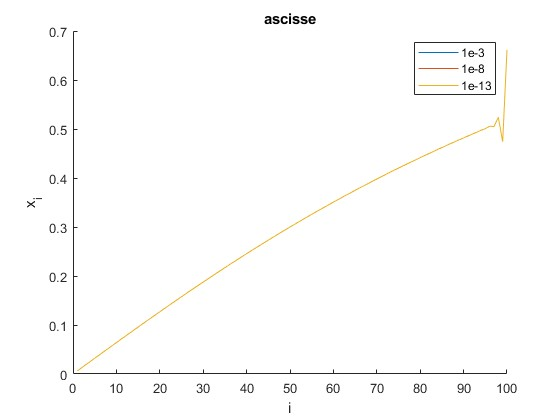
\includegraphics[width=\textwidth]{asc15.jpg}
    \end{minipage}
    \begin{minipage}[b]{0.48\textwidth}
        \centering
        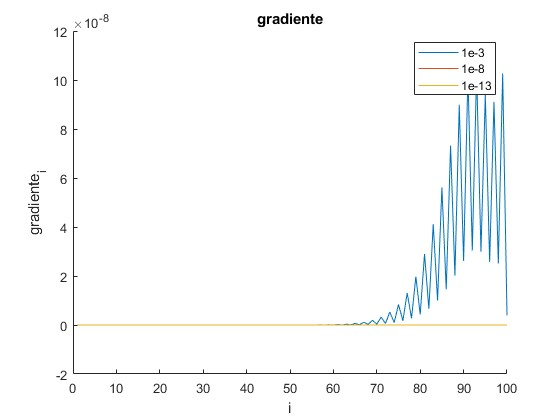
\includegraphics[width=\textwidth]{gra15.jpg}
    \end{minipage}
\end{figure}
Come si può notare dai grafici usando le tolleranze \texttt{1e-8}, \texttt{1e-13} si ottiene che il gradiente è quasi nullo, ovvero le ascisse \(x_i\) risultano essere un punto stazionario.
Tabulando infatti la norma 2 dei gradienti con le tolleranze si ha:
\begin{center}
    \begin{tabular}{||c | c ||} 
         \hline      
         tol & norma del gradiente\\
         \hline
         1e-2 & 2.70412063725952e-07 \\
         \hline
         1e-08 & 1.55513291374585e-15 \\
         \hline
         1e-13 & 1.55513291374585e-15 \\
         \hline
    \end{tabular}
    \end{center}
\newpage
\begin{tcolorbox}
\paragraph{Esercizio 16:}
Costruire una function, \texttt{lagrange.m}, avente la stessa sintassi della function \texttt{spline}
di Matlab, che implementi, in modo vettoriale, la forma di Lagrange del polinomio interpolante una
funzione.
\end{tcolorbox}
\paragraph{Soluzione:}

\texttt{CODICE Matlab per funzione Lagrange}
\begin{lstlisting}[frame=single]
function p = lagrange(x, y, xq)
%
%   p=lagrange(x, y, xq)
%
%   Calcolo del polinomio interpolante in base di Lagrange:
%
%   Input:
%   x: ascisse di interpolazione
%   y: valori della funzione interpolanda nelle ascisse di interpolazione
%   xq: valori su cui calcolare il valore del polinomio interpolante
%
%   Output:
%   p: vettore con i valori calcolati
%
n=length(x);
if length(unique(x))~=n
    error("Le ascisse non sono distinte tra loro");
end
if length(y)~=n
    error("I vettori x ed y devono avere la stessa lunghezza");
end
p=zeros(size(xq));
for i=1:n
    p=p+y(i)*Lin(i,x,xq);
end
return
end
\end{lstlisting}
\texttt{CODICE Matlab per funzione Lin}

\begin{lstlisting}[frame=single]
function L = Lin(i, xi, x)
%
%   L=Lin(i,xi,x)
%
%   Calcolo della base di Lagrange
%
%   Input:
%   i: indice
%   xi: ascisse di interpolazione
%   x: valori su cui calcolare la base di Lagrange
%
%   Output:
%   L: vettore con i valori della base di Lagrange con indice i
%
L=ones(size(x));
zi=xi(i);
xi(i)=[];
n=length(xi);
for j=1:n
    L=L.*(x-xi(j));
end
L=L/prod(zi-xi);
return
end
\end{lstlisting}

\begin{tcolorbox}
\paragraph{Esercizio 17:}
Costruire una function, \texttt{newton.m}, avente la stessa sintassi della function \texttt{spline}
di Matlab, che implementi, in modo vettoriale, la forma di Newton del polinomio interpolante una
funzione.
\end{tcolorbox}
\paragraph{Soluzione:}

\texttt{CODICE Matlab per funzione Newton}
\begin{lstlisting}[frame=single]
function p = newton(x, y, xq)
%
%   p=newton(x, y, xq)
%
%   Calcolo del polinomio interpolante in base di Newton:
%
%   Input:
%   x: ascisse di interpolazione
%   y: valori della funzione interpolanda nelle ascisse di interpolazione
%   xq: valori su cui calcolare il valore del polinomio interpolante
%
%   Output:
%   p: vettore con i valori calcolati
%
n = length(x)-1;
if length(unique(x))~=n+1
    error("Le ascisse non sono distinte tra loro");
end
if length(y)~=n+1
    error("I vettori x ed y devono avere la stessa lunghezza");
end
for j=1:n
    for i=n+1:-1:j+1
        y(i)=(y(i)-y(i-1))/(x(i)-x(i-j));
    end
end
p=horner(x,y,xq);
return
end
\end{lstlisting}
\texttt{CODICE Matlab per l'algoritmo di Horner}
\begin{lstlisting}[frame=single]
function p = horner(x, f, xq)
%
%   p=horner(x, f, ,xq)
%
%   Algoritmo di horner generalizzato per il calcolo di un polinomio:
%
%   Input:
%   x: ascisse di interpolazione
%   f: valori delle differenze divise
%   xq: valori su cui calcolare il polinomio
%
%   Output:
%   p: vettore con i valori calcolati
%
n=length(x)-1;
p=ones(size(xq))*f(n+1);
for i=n:-1:1
    p=p.*(xq-x(i))+f(i);
end
return
end
\end{lstlisting}

\begin{tcolorbox}
\paragraph{Esercizio 18:}
Costruire una function, \texttt{hermite.m}, avente sintassi
\begin{center}
    \texttt{yy = hermite( xi, fi, f1i, xx )}
\end{center}
che implementi, in modo vettoriale, il polinomio interpolante di Hermite.
\end{tcolorbox}
\paragraph{Soluzione:}

\texttt{CODICE Matlab per hermite}
\begin{lstlisting}[frame=single]
function yy = hermite(xi, fi, f1i, xx)
%
%   p=hermite(xi, fi, ,f1i, xx)
%
%   Calcolo del polinomio interpolante di Hermite:
%
%   Input:
%   xi: ascisse di interpolazione
%   fi: valori della funzione interpolanda nelle ascisse di interpolazione
%   f1i: valori della derivata prima della funzione interpolanda nelle
%   ascisse di interpolazione
%   xx: valori su cui calcolare il valore del polinomio interpolante
%
%   Output:
%   yy: vettore con i valori calcolati
%
n=length(xi)-1;
if length(unique(xi))~=n+1
    error("Le ascisse non sono distinte tra loro");
end
if length(fi)~=n+1 || length(f1i)~=n+1
    error("I vettori xi, fi e f1i devono avere la stessa lunghezza");
end
xi=repelem(xi,2);
fi=repelem(fi,2);
fi(2:2:end)=f1i;
for i = (2*n+1):-2:3
    fi(i)=(fi(i)-fi(i-2))/(xi(i)-xi(i-1));
end
for j=2:2*n+1
    for i = (2*n+2):-1:j+1
        fi(i)= (fi(i)-fi(i-1))/(xi(i)-xi(i-j));
    end
end
yy=horner(xi,fi,xx);
return
end
\end{lstlisting}
\texttt{CODICE Matlab per l'algoritmo di horner}
\begin{lstlisting}[frame=single]
function p = horner(x, f, xq)
%
%   p=horner(x, f, ,xq)
%
%   Algoritmo di horner generalizzato per il calcolo di un polinomio:
%
%   Input:
%   x: ascisse di interpolazione
%   f: valori delle differenze divise
%   xq: valori su cui calcolare il polinomio
%
%   Output:
%   p: vettore con i valori calcolati
%
n=length(x)-1;
p=ones(size(xq))*f(n+1);
for i=n:-1:1
    p=p.*(xq-x(i))+f(i);
end
return
end

\end{lstlisting}
\begin{tcolorbox}
\paragraph{Esercizio 19:}
Costruire una function Matlab che, specificato in ingresso il grado \emph{n} del polinomio
interpolante, e gli estremi dell'intervallo [\emph{a}, \emph{b}], calcoli le corrispondenti ascisse di Chebyshev.
\end{tcolorbox}
\paragraph{Soluzione:} Calcolo delle ascisse di Chebyshev 
\begin{lstlisting}[frame=single]
function x = cheby(n,a,b)
%
%   x=cheby(n,a,b)
%
%   Calcolo delle ascisse di Chebyshev:
%
%   Input:
%   n: grado del polinomio
%   a,b: estremi dell'intervallo
%
%   Output:
%   x: vettore contentente le ascisse di Chebyshev
if n<=0 || n~=fix(n)
    error('n deve essere un numero naturale');
elseif a>=b
    error('l''intervallo non e'' corretto');
end
x=(a+b)/2 + cos((2*(n:-1:0)+1)*pi./(2*(n+1))) * (b-a)/2;
return
end
\end{lstlisting}
\newpage
\begin{tcolorbox}
\paragraph{Esercizio 20:}
Costruire una function Matlab, con sintassi
\begin{center}
    \texttt{ll = lebesgue( a, b, nn, type )}
\end{center}
che approssimi la costante di Lebesgue per l'interpolazione polinomiale sull'intervallo \texttt{[a,b]}, per
i polinomi di grado specificato nel vettore \texttt{nn}, utilizzando ascisse equidistanti, se \texttt{type=0}, o di
Chebyshev, se \texttt{type=1} (utilizzare 10001 punti equispaziati nell'intervallo \texttt{[a,b]} per ottenere ciascuna componente di ll). 
Graficare i risultati ottenuti, per \texttt{nn=1:100}, utilizzando \texttt{[a,b]=[0,1]} e \texttt{[a,b]=[-3,7]}. Giustificare i risultati ottenuti.
\end{tcolorbox}
\paragraph{Soluzione:} Calcolo della costate di Lebesgue:

\begin{lstlisting}[frame=single]
function ll = lebesgue(a,b,nn,type)
%
%   ll = lebesgue(a,b,nn,type)
%   Calcola un'approssimazione della costante di Lebesgue per 
%   l'interpolazione polinomiale sull'intervallo [a,b]
%
%   Input:
%   a,b: estremi intervallo
%   nn: grado dei polinomi
%   type: 
%       0 - ascisse equidistanti
%       1 - ascisse di Chebyshev
%   Output:
%   ll: approssimazione costante di Lebesgue ottenuta   
%
if nargin<4
    error("inserire tutti i dati");
end
if a>b
    error('a deve essere piu piccolo di b');
end
n=length(nn);
ll=zeros(1,length(nn));
f=0;
if type==1
    f=@(n) cheby(n,a,b);
elseif type==0
    f=@(n) linspace(a,b,n+1);
end
for i=1:n
    xi=f(nn(i));
    x=linspace(a,b,10001);
    L=zeros(size(x));
    for j=1:length(xi)
        L=L+abs(Lin(j,xi,x));
    end
    ll(i)=max(L);
end
return
end
\end{lstlisting}
Graficando i risulati della funzione eseguita sugli intervalli [0,1] e [-3,7] con type=0 e type=1 si ottiene:
\begin{figure}[H]
    \begin{minipage}{0.5\textwidth}
      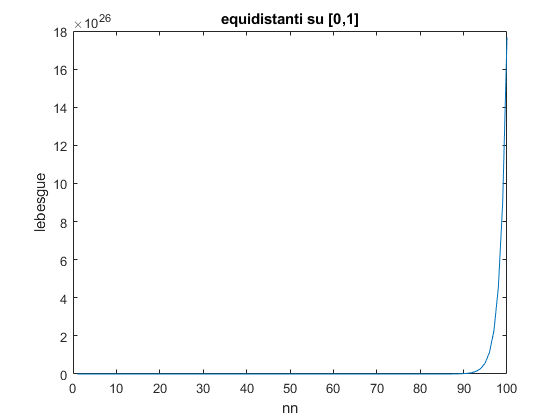
\includegraphics[width=\linewidth]{01e.png}
    \end{minipage}
    \begin{minipage}{0.5\textwidth}
      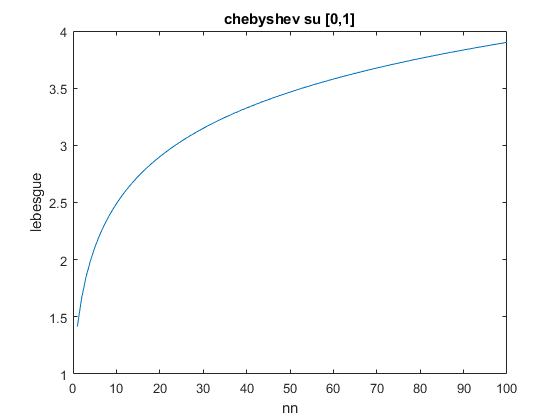
\includegraphics[width=\linewidth]{01c.png}
    \end{minipage}
    \begin{minipage}{0.5\textwidth}
        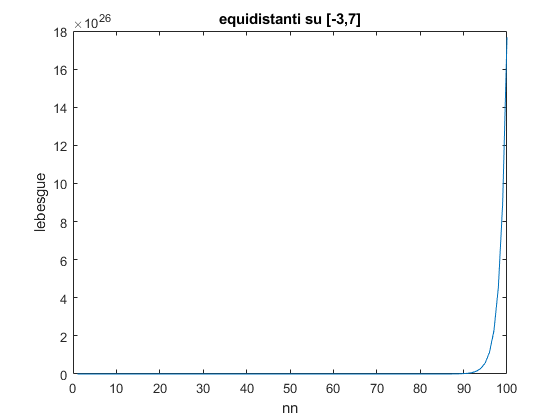
\includegraphics[width=\linewidth]{37e.png}
      \end{minipage}
      \begin{minipage}{0.5\textwidth}
        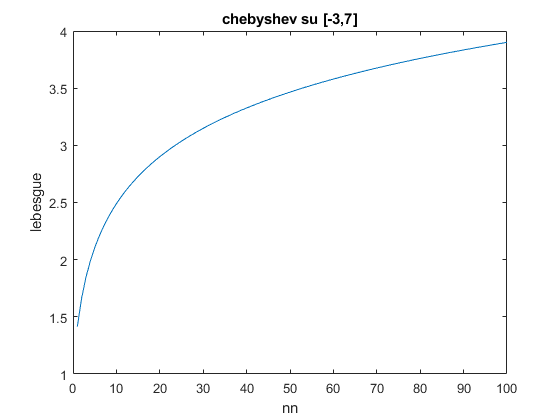
\includegraphics[width=\linewidth]{37c.png}
      \end{minipage}
 \end{figure}
Si può vedere come la costante di lebesgue cresca molto velocemente quando vengono usate ascisse equidistanti rispetto alle ascisse di chebyshev. 
D'altronde \(\Lambda\) cresce almeno come \(O(logx)\), infatti usando ascisse equidistanti
 si ottiene una crescita esponenziale rispetto a quella ottimale ottenuta 
 mediante le ascisse di Chebyshev \(\Lambda \approx O(logx)\), come si può notare dal grafico.
 \newpage
 \begin{tcolorbox}
\paragraph{Esercizio 21:}
Utilizzando le function dei precedenti esercizi, graficare (in semilogy) l'andamento
errore di interpolazione (utilizzare 10001 punti equispaziati nell'intervallo per ottenerne la stima)
per la funzione di Runge,
\begin{equation}
    f(x)=\frac{1}{1+x^{2}}, \hspace{1cm} x \in [-5,5]
\end{equation}

utilizzando sia le ascisse equidistanti che di Chebyshev, per i polinomi interpolanti di grado \texttt{nn=2:2:100}.
Graficare l'errore di interpolazione anche per i polinomi interpolanti di Hermite di grado \texttt{nn=3:2:99},
sia utilizzando ascisse equidistanti che ascisse di Chebyshev, nell'intervallo considerato.
\end{tcolorbox}
\paragraph{Soluzione:}
Stimando l'errore con la norma infinito su 10001 punti si ottiene per Lagrange:
\begin{figure}[H]
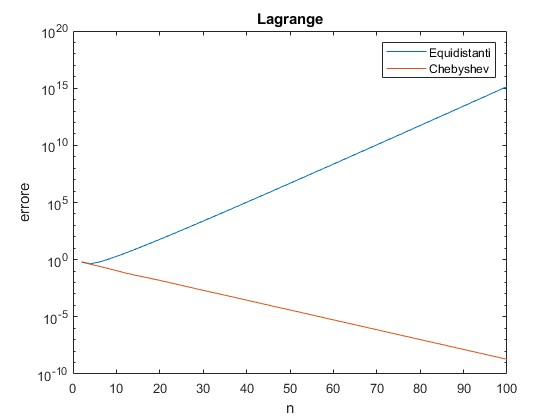
\includegraphics[width=0.7\textwidth]{lag21.jpg}
\end{figure}
\newpage
Per Newton invece si ottiene:
\begin{figure}[H]
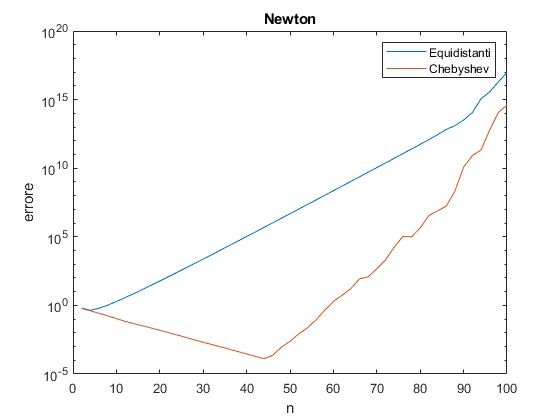
\includegraphics[width=0.7\textwidth]{new21.jpg}
\end{figure}
E similmente per Hermite si ottiene:
\begin{figure}[H]
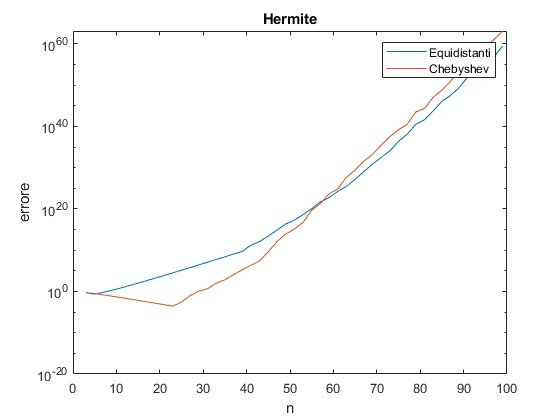
\includegraphics[width=0.7\textwidth]{her21.jpg}
\end{figure}
\newpage
\begin{tcolorbox}
\paragraph{Esercizio 22:}
Costruire una function, \texttt{myspline.m}, avente sintassi
\begin{center}
\texttt{yy = myspline( xi, fi, xx, type )}
\end{center}

dove \texttt{type=0} calcola la \emph{spline} cubica interpolante naturale i punti \texttt{(xi,fi)}, e \texttt{type\textasciitilde=0} calcola quella calcola quella
\emph{not-a-knot} (default).
\end{tcolorbox}
\paragraph{Soluzione:} \texttt{CODICE Matlab spline cubica}
\begin{lstlisting}[frame=single]
function yy = myspline(xi,fi,xx,type)
%
% yy=myspline(xi,fi,xx,type)
%
% Calcolo dei valori della spine interpolante le ascisse
%
%
% Input:
% xi: vettori con le ascisse di interpolazione
% fi: vettore con i valori della funzione per le ascisse
% xx: vettore con i valori su cui calcolare la spline
% type: 0 per la spline naturale, diverso da 0 per not-a-knot (default)
%
% Output:
% yy: vettore con i valori della spline calcolati 
%
n=length(xi)-1;
if length(unique(xi))~=n+1
    error("Le ascisse non sono distinte tra loro");
end
if length(fi)~=n+1
    error("I vettori xi ed fi devono avere la stessa lunghezza");
end
h=zeros(1,n);
df=fi;
if nargin<4
    type=1;
end
for j=1:2 %differenze divise
    for i=n+1:-1:j+1
        df(i)=(df(i)-df(i-1))/(xi(i)-xi(i-j));
    end
end
h=xi(2:n+1)-xi(1:n);
phi(1:n-1)=h(1:n-1)./(h(1:n-1)+h(2:n));
eps(1:n-1)=h(2:n)./(h(1:n-1)+h(2:n));
m(1:n-1)=df(3:n+1)*6;
b=phi(2:n-1);
a=2*ones(1,n-1);
c=eps(1:n-2);
if type~=0 %cambio della prima riga e ultima riga per not-a-knot
    m(1)=m(1)*(1-phi(1));
    m(n-1)=m(n-1)*(1-eps(n-1));
    c(1)=c(1)-phi(1);
    a(1)=a(1)-phi(1);
    b(n-2)=b(n-2)-eps(n-1);
    a(n-1)=a(n-1)-eps(n-1);
end
%risoluzione matrice tridiagonale
for i=1:n-2
    b(i)=b(i)/a(i);
    a(i+1)=a(i+1)-b(i)*c(i);
    m(i+1)=m(i+1)-b(i)*m(i);   
end
m(n-1)=m(n-1)/a(n-1);
for i=n-2:-1:1
    m(i)=(m(i)-c(i)*m(i+1))/a(i);
end
%condizioni spline naturale e not-a-knot
if type==0
    m= [0 m 0];
else
    m = [df(3)-m(1)-m(2), m ,df(n+1)-m(n-1)-m(n-2)];
end
%calcolo di r e q
r=zeros(1,n);
q=zeros(1,n);
for i=1:n
    r(i)=fi(i)-((h(i)^2)/6)*m(i);
    q(i)=(fi(i+1)-fi(i))/h(i)-(h(i)/6)*(m(i+1)-m(i));
end
%calcolo spline
yy=zeros(1,length(xx));
for i=1:length(xx)
    for k=1:n
        if xx(i)>=xi(k) && xx(i)<=xi(k+1)
            yy(i)=(((xx(i)-xi(k))^3)*m(k+1)+((xi(k+1)-xx(i))^3)*m(k))/( ...
                6*h(k))+q(k)*(xx(i)-xi(k))+r(k);
            break
        end
    end
end
return
end
\end{lstlisting}
\newpage
\begin{tcolorbox}
\paragraph{Esercizio 23:}
Graficare, utilizzando il formato semilogy, l'errore di approssimazione utilizzando le
\emph{spline} interpolanti naturale e \emph{not-a-knot} per approssimare la funzione di Runge sull'intervallo [-5,5],
utilizzando una partizione \(\Delta = \{-5=x_0 <...<x_n=5\}\), con ascisse equidistanti e \texttt{n=4:4:400}.
Utilizzare 10001 punti equispaziati nell'intervallo \text{[-5, 5]} per ottenere la stima dell'errore.
\end{tcolorbox}
\paragraph{Soluzione:}
Graficando la norma infinito per 10001 per stimare l'errore di interpolazione si ottiene:
\begin{figure}[H]
    \begin{minipage}{0.5\textwidth}
      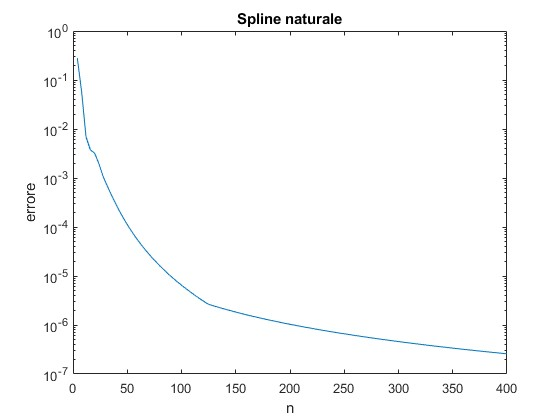
\includegraphics[width=\linewidth]{snaturale.jpg}
    \end{minipage}
    \begin{minipage}{0.5\textwidth}
      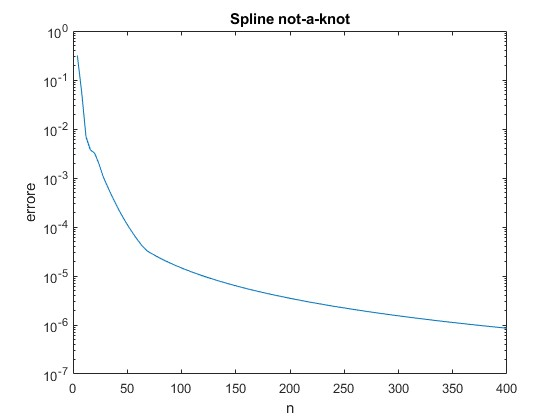
\includegraphics[width=\linewidth]{sknot.jpg}
    \end{minipage}
 \end{figure}
E' possibile notare come, rispetto ai polinomi interpolanti, l'errore diminuisce all'aumentare delle ascisse equidistanti.
\begin{tcolorbox}
\paragraph{Esercizio 24:}
E' noto che un fenomeno fisico evolve come \(y = x^{n}\) con \emph{n} incognito. 
Il file \texttt{data.mat} contiene 1000 coppie di dati \((x_{i},y_{i})\), in cui la seconda componente è affetta da un errore con distribuzione Gaussiana a media nulla e varianza “piccola”. Utilizzando un opportuno polinomio
di approssimazione ai minimi quadrati, stimare il grado \emph{n}. Argomentare il procedimento seguito,
graficando la norma del residuo rispetto a valori crescenti di \emph{n}. E richiesto il codice Matlab dell'algoritmo 
che avrete implementato (potete utilizzare, se lo ritenete opportuno, la function \texttt{polyfit}
di Matlab).
\end{tcolorbox}
\paragraph{Soluzione:} 
Dato che l'incognita dell'equazione è l'esponente, conviene innanzitutto riscriverla utilizzando le proprietà dei logaritmi: \\
$$ y=x^{n} \Rightarrow ln(y)=ln(x^{n}) \Rightarrow ln(y)=nln(x)$$
Così facendo si ottiene una equazione lineare che una volta applicata alle coppie \((x_i,y_i)\) delle misurazioni 
permette di utilizzare un'approsimazione polinomiale ai minimi quadrati di grado 1 per stimare il valore di \texttt{n} che sarà dato dal coefficente \(a_1\). 
Per meglio transformare i dati in modo che si avvicinino una retta, conviene usare una rappresentazione in scala semi-logaritmica,
 si potrebbe infatti approssimare \(ln(x)\) con la retta tangente al punto \(x_{0}=1\) ottenendo così:
\(ln(y) \approx n(x-1)\). Un'ulteriore considerazione da fare è quella di scartare le misurazioni \(y_i\) negative, 
essendo le ascisse \(x_i\) tutte positive e di conseguenza anche \(x_i^{n}\), ed inoltre non sarebbe possibile calcolare \(log(y)\).
\newpage
L'algoritmo descritto è stato così implementato:
\begin{lstlisting}[frame=single]
function n = estimate(data)
%
% n = estimate(data)
%
% Stima il grado di n date m coppie di dati per y=x^n
%
%
% Input:
% data: matrice mx2 con le misurazioni del problema
%
% Output:
% n: grado stimato del polinomio
%
fixedData=data;
fixedData(fixedData(:,2)<0,:)=[];
x=fixedData(:,1);
y=log(fixedData(:,2));
r=polyfit(x,y,1);
n=r(1);
return
end
\end{lstlisting}
Si ottiene quindi che il grado \texttt{n} è 5, come si può notare graficando in \texttt{semilogy} l'errore (approsimato con la norma 2) del residuo rispetto ad n: \\
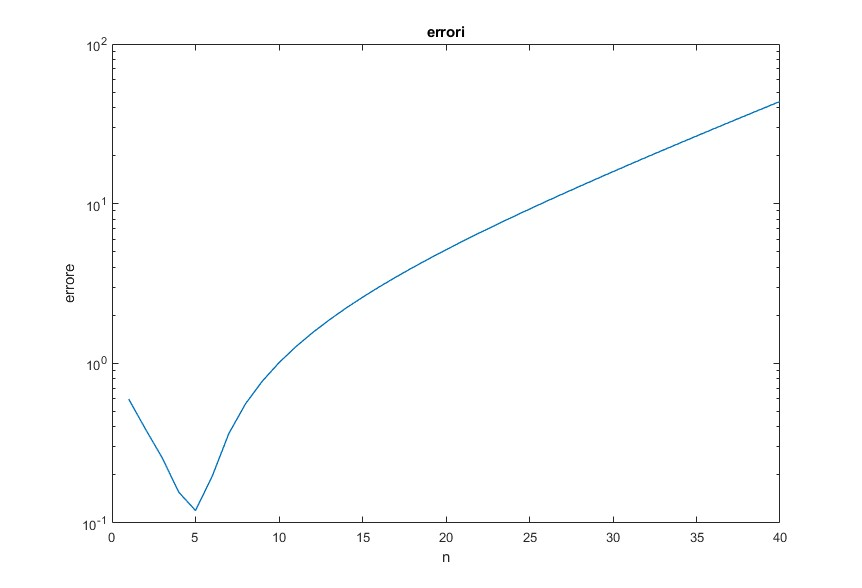
\includegraphics[width=0.7\textwidth]{errori24.jpg} \\
difatti esso è minimo per \texttt{n=5}.
\newpage
\begin{tcolorbox}
\paragraph{Esercizio 25:}
Costruire una function Matlab che, dato in input \emph{n}, restituisca i pesi della quadratura della formula di Newton-Cotes di grado \emph{n}. Tabulare, quindi, i pesi delle formule di grado
1, 2,. . . , 7 e 9 (come numeri razionali).
\end{tcolorbox}

\paragraph{Soluzione:}

\texttt{codice per i pesi di Newton Codes}
\begin{lstlisting}[frame=single]
function c = pesiNewtCotes(n)
%
%   c=pesiNewtCotes
%
%   Calcolo dei pesi della formula di Newton Cotes:
%
%   Input:
%   n: grado della formula
%
%   Output:
%   c: vettore con i pesi
%
if n<1 || n~=fix(n)
    error('n deve essere un numero naturale');
else
c=zeros(1,n);
for i=0:n/2
    den = prod( i - [0:i-1, i+1:n]);
    coeff = poly([0:i-1 i+1:n]);
    coeff = [coeff./((n+1):-1:1) 0];
    num=polyval(coeff,n);
    c(i+1)=num/den;
end
for i=n+1:-1:n/2
    c(i) = c(n+2-i);
end
return
end
\end{lstlisting}


\begin{center}
\begin{adjustbox}{width=\textwidth}
\begin{tabular}{||c || c | c | c | c | c | c | c | c | c | c ||} 
     \hline
     
     n & 0 & 1 & 2 & 3 & 4 & 5 & 6 & 7 & 8 & 9\\
     \hline\hline
     1 & 1/2 & 1/2 & & & & & & & &\\ 
     \hline
     2 & 1/3 & 4/3 & 1/3 & & & & & & &\\
     \hline
     3 & 3/8 & 9/8 & 9/8 & 3/8 & & & & & &\\
     \hline
     4 & 14/45 & 64/45 & 8/15 & 64/45 & 14/45 & & & & &\\
     \hline
     5 & 95/288 & 125/96 & 125/144 & 125/144 & 125/96 & 95/288 & & & &\\ 
     \hline
     6 & 41/140 & 54/35 & 27/140 & 68/35 & 27/140 & 54/35 & 41/140 & & &\\  
     \hline
     7 & 1073/3527 & 810/559 & 343/640 & 649/536 & 649/536 & 343/640 & 810/559 & 1073/3527 & &\\  
     \hline
     9 & 130/453 & 1374/869 & 243/2240 & 5287/2721 & 704/1213 & 704/121 & 5287/2721 & 243/2240 & 1374/869 & 130/453\\
     \hline
\end{tabular}
\end{adjustbox}
\end{center}


\begin{tcolorbox}
\paragraph{Esercizio 26:}
Scrivere una function Matlab, \\

\texttt{[If,err] = composita( fun, a, b, k, n )}

che implementi la formula composita di Newton-Cotes di grado \texttt{k} su \texttt{n+1} ascisse equidistanti, con \texttt{n}
multiplo pari di \texttt{k}, in cui:

\begin{itemize}
    \item \texttt{fun} è la funzione integranda (che accetta input vettoriali);
    \item \texttt{[a,b]} è l’intervallo di integrazione;
    \item \texttt{k}, \texttt{n} come su descritti;
    \item \texttt{If} è l’approssimazione dell’integrale ottenuta;
    \item \texttt{err} è la stima dell’errore di quadratura.
\end{itemize}
\end{tcolorbox}
\paragraph{Soluzione:} Calcolo della formula composita di Newton-Cotes di grado \texttt{k} su \texttt{n+1} ascisse equidistanti.
\begin{lstlisting}[frame=single]
function [If,err] = composita(fun, a, b, k, n)
%
%   [If,err] = composita(fun,a,b,k,n)
%
%   Stima dell'integrale definito cone le formule composite di Newton-Cotes
%
%   Input:
%   fun: funzione integrale
%   a : lato destro intervallo di integrazione 
%   b: lato destron intervallo di integrazione
%   k: grado della formula di Newton-Cotes
%   n: numero di punti da usare (deve essere un multiplo pari di k)
%
%   Output:
%   If: valore dell'integrale
%   err: stima dell'errore
%
if a==b
    If=0;
    err=0;
    return
end
if a>b
    error('intervallo non corretto');
end
if mod((n/k),2)~=0
    error('n deve essere un multiplo pari di k');
end
x=linspace(a,b,n+1);
y=fun(x);
h=(b-a)/n;
c=pesiNewtCotes(k);
If=0;
for i=1:k:n+1-k
    If=If+sum(y(i:i+k).*c);
end
If=h*If;
IfH=0;
for i=1:2*k:n+1-2*k
    IfH=IfH+sum(y(i:2:i+2*k).*c);
end
IfH=2*h*IfH;
u = 2-mod(k,2);
err=abs(IfH-If)/(2^(k+u)-1);
return
\end{lstlisting}

\begin{tcolorbox}
\paragraph{Esercizio 27:}
Utilizzare la function \texttt{composita} per ottenere l’approssimazione dell’integrale\\
$$\int_{0}^{1}(\sum_{i=1}^{5}i\cos(2\pi{ix})-e^{i}\sin(2(\pi{i}+0.1)x))dx$$
con le formule composite di Newton-Cotes di grado \texttt{k=1,2,3,6}. Per tutte, utilizzare \texttt{n=12}.
\end{tcolorbox}
\paragraph{Soluzione:}

Utilizzando le formule composite di Newton-Cotes con n=12 per approssimare l'integrale si vanno ad ottenere i seguenti risultati: \\

\begin{center}
    \begin{tabular}{||c || c | c ||} 
        \hline
        k & valore & errore \\
        \hline
        \hline
        1 & -0.092598047616972 & 0.192379444267582 \\
        \hline
        2 & -0.284977491884554 & 0.034967622162555 \\
        \hline
        3 & 0.114030927423084 & 0.029823785706593 \\
        \hline
        6 & -0.702525851480416 & 0.002428474323110 \\
        \hline
    \end{tabular}
    \end{center}
Si può notare come i risultati risultano essere imprecisi e discordanti tra loro, infatti andando a graficare la funzione in esame negli estremi dell'intervallo di integrazione \\
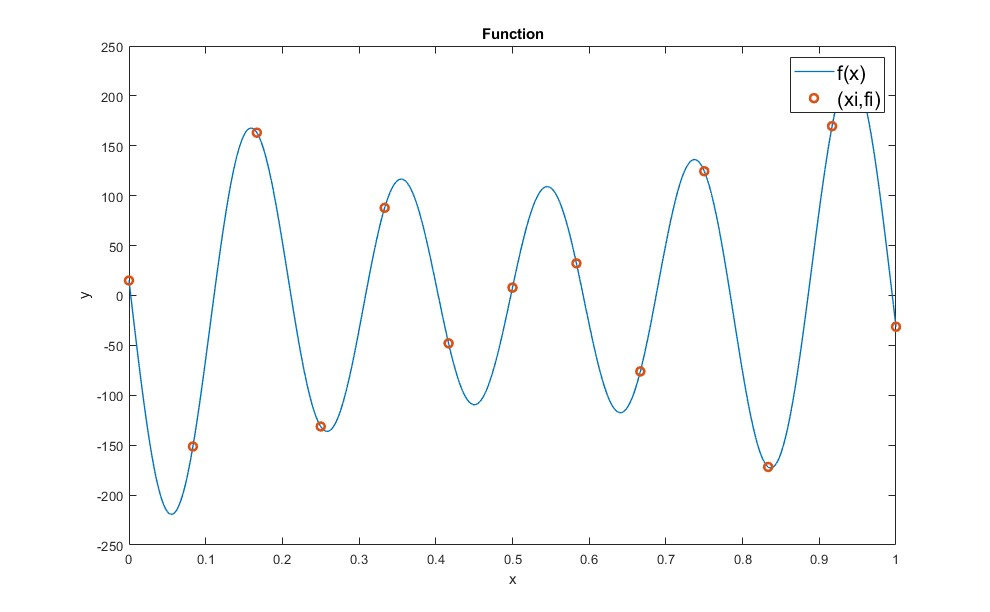
\includegraphics[width=\linewidth]{plot27.jpg}
possiamo notare che oscilla frequentemente, rendendo le formule più inaccurate per le ascisse considerate.
Aumentando il numero di quest'ultime si può ridurre ulteriormente l'errore, d'altronde si ha:
$$E_k^{(n)} = v_k f^{(k+u)}(\xi)\biggl(\frac{b-a}{k}\biggr)\biggl(\frac{b-a}{n}\biggr)^{(k+u)} con  \xi \in [a,b]$$
che sappiamo tende a 0 per n che tende ad infinito, altrimenti si possono usare pure le formule adattive.

\begin{tcolorbox}
\paragraph{Esercizio 28:}
Implementare la formula composita adattativa di Simpson.
\end{tcolorbox}
\paragraph{Soluzione:} Calcolo della formula adattiva di Simpson
\begin{lstlisting}[frame=single]
function [I2,vf] = adapsim(a,b,f,tol,fa,f1,fb)
%
%   [I2,vf] = adapsim(a,b,f,tol)
% 
%   Calcola la formula adattiva di Simpson
%
%   Input:
%   a,b: estremi intervallo di integrazione
%   f: function funzione integranda
%   tol: tolleranza richiesta
%   Output:
%   I2: approssimazione ottenuta
%   vf: valutazioni funzionali
%
if a==b
    I2=0;
    return
elseif a>b
    error('intervallo non corretto');
elseif tol<0
    error('tolleranza negativa');
end
x1=(a+b)/2;
vf=0;
if nargin==4
    fa=feval(f,a);
    fb=feval(f,b);
    f1=feval(f,x1);
    vf=3;
end
h=(b-a)/6;
I1=h*(fa+4*f1+fb);
x2=(a+x1)/2;
x3=(x1+b)/2;
f2=feval(f,x2);
f3=feval(f,x3);
I2=.5*h*(fa+4*f2+2*f1+4*f3+fb);
vf=vf+2;
e=abs(I2-I1)/15;
if e>tol
    [left,vf1]=adapsim(a,x1,f,tol/2,fa,f2,f1);
    [right,vf2]=adapsim(x1,b,f,tol/2,f1,f3,fb);
    I2=left+right;
    vf=vf+vf1+vf2;
end
return
end
\end{lstlisting}

\newpage
\begin{tcolorbox}
\paragraph{Esercizio 29:}
Implementare la formula composita adattativa di Newton-Cotes di grado \texttt{k=4}.
\end{tcolorbox}
\paragraph{Soluzione:} Calcolo della formula adattiva di Newton-Cotes di grado k=4.
\begin{lstlisting}[frame=single]
function [I2,vf] = adapquad(a,b,f,tol,fa,f1,f2,f3,fb)
%
%   [I2,vf] = adapquad(a,b,f,tol)
% 
%   Calcola la formula adattiva di Simpson
%
%   Input:
%   a,b: estremi intervallo di integrazione
%   f: function funzione integranda
%   tol: tolleranza richiesta
%   Output:
%   I2: approssimazione ottenuta
%   vf: valutazioni funzionali
%
if a==b
    I2=0;
    return
elseif a>b
    error('intervallo non corretto');
elseif tol<0
    error('tolleranza negativa');
end
vf=0;
x2=(a+b)/2;
x1=(a+x2)/2;
x3=(x2+b)/2;
if nargin==4
    fa=feval(f,a);
    fb=feval(f,b);
    f1=feval(f,x1);
    f2=feval(f,x2);
    f3=feval(f,x3);
    vf=5;
end
h=(b-a)/180;
I1=h*(14*fa+64*f1+24*f2+64*f3+14*fb);
x4=(a+x1)/2;
x5=(x1+x2)/2;
x6=(x2+x3)/2;
x7=(x3+b)/2;
f4=feval(f,x4);
f5=feval(f,x5);
f6=feval(f,x6);
f7=feval(f,x7);
I2=.5*h*(14*fa+64*f4+24*f1+64*f5+28*f2+64*f6+24*f3+64*f7+14*fb);
vf=vf+4;
e=abs(I2-I1)/63;
if e>tol
    [left,vf1]=adapquad(a,x2,f,tol,fa,f4,f1,f5,f2);
    [right,vf2]=adapquad(x2,b,f,tol,f2,f6,f3,f7,fb);
    I2=left+right;
    vf=vf+vf1+vf2;
end
return
end
\end{lstlisting}


\newpage
\begin{tcolorbox}
\paragraph{Esercizio 30:}
Confrontare le formule adattative degli ultimi due esercizi, tabulando il numero
di valutazioni funzionali effettuate, rispetto alla tolleranza \texttt{tol = 1e-2, 1e-3, ..., 1e-9}, per
ottenere l’approssimazione dell’integrale \\
$$\int_{10^{-5}}^{1}x^{-1}\cos(\log(x^{-1}))dx\equiv\sin(\log(10^{5}))$$
Costruire un’altra tabella, in cui si tabula l’errore vero (essendo l’integrale noto, in questo caso)
rispetto a \texttt{tol}.
\end{tcolorbox}
\paragraph{Soluzione:}
Tabulando le valutazioni funzionali si ottiene:
\begin{center}
\begin{tabular}{||c || c | c ||} 
    \hline
    tol &  valutazioni funzionali n=2 & valutazioni funzionali n=4 \\
    \hline
    \hline
    1e-2 & 201 & 113 \\
    \hline
    1e-3 & 333 & 121 \\
    \hline
    1e-4 & 605 & 129 \\
    \hline
    1e-5 & 1061 & 137 \\
    \hline
    1e-6 & 1869 & 145 \\
    \hline
    1e-7 & 3277 & 265 \\
    \hline
    1e-8 & 5921 & 345 \\
    \hline
    1e-9 & 10589 & 473 \\
    \hline
\end{tabular}
\end{center}
Mentre tabulando l'errore effettivo si ottiene:
\begin{center}
    \begin{tabular}{||c || c | c | c | c ||} 
        \hline
         &  \multicolumn{2}{|c|}{n=2} & \multicolumn{2}{|c|}{n=4}\\
         \hline
        tol & valore & errore & valore & errori \\
        \hline
        \hline
        1e-2 & -0.869425809078715 & 2.935280256943784e-04 & -0.818445828479865 & 0.050686452573156 \\
        \hline
        1e-3 & -0.869589504976433 & 4.572239234117426e-04 & -0.863917726701441 & 0.005214554351580 \\
        \hline
        1e-4 & -0.869158635812636 & 2.635475961443312e-05 & -0.868851170727444 & 2.811103255769831e-04 \\
        \hline
        1e-5 & -0.869134625866697 & 2.344813675669855e-06 & -0.869126106965213 & 6.174087807786499e-06 \\
        \hline
        1e-6 & -0.869132581815646 & 3.007626251383400e-07 & -0.869134425591871 & 2.144538849502276e-06  \\
        \hline
        1e-7 & -0.869132317617779 & 3.656475811020243e-08 & -0.869132234992719 & 4.606030246101511e-08 \\
        \hline
        1e-8 & -0.869132284264119 & 3.211098165145643e-09 & -0.869132276557698 & 4.495323446818134e-09 \\
        \hline
        1e-9 & -0.869132281362861 & 3.098394874001542e-10 & -0.869132278121886 & 2.931135223427361e-09 \\
        \hline
    \end{tabular}
    \end{center}
Da cui si può notare che le valutazioni funzionali per Simpson sono molto maggiori per le formule adattive con \texttt{n=4}, tuttavia con \texttt{n=2} si riesce a raggiungere un errore inferiore rispetto all'altra formula a parità di tolleranza.
\end{document}